
\chapter{A Taste of Their Own Medicine: A.I.T. and The Evidence}\label{intro}

\Authorline{Shivashankar Sastry}


\section*{Abstract}

The so called “Aryan Invasion (or Migration) theory” was constructed out of mistranslations and misinterpretations of Sanskrit texts and used to promote a racist nineteenth and early twentieth century agenda. Once the theory was established as “mainstream knowledge,” evidence was either produced or concocted to fit in with the theory. This paper is in three parts. Part 1 argues that Aryans and Dravidian never existed, that they were concoctions of racist European philologists and provides the evidence to support this view. Part 2 explores the reason why it became vitally important for European scholars to lay claim on the Sanskrit language and try and find a route for the language to have come from somewhere closer to Europe than anywhere else. Part 3 deals with the utility, or lack of utility of genetics in figuring out the language that people spoke and the actual age of the Indian genome compared with the Aryan migration theory.


\section*{Part 1}

Peoples and nations recall their past in various ways. Very old civilizations may have oral narratives like the Indian purāņa-s, or the narratives of Red Indians and Australian aborigines. Later civilizations maintained written documents such as the Greek historians. In other instances the past can be surmised and guessed from archaeological remains. Accounts of contemporary travelers such as Xuanzang (Hiuen Tsang), Al Beruni and Marco Polo add to our knowledge of the past. Sometimes archaeological findings have an unexpected correlation with existing texts – like the Assyrian ruins of the Levant being recalled in Biblical texts.

But India must be the only country on earth to have its history invented and told to us by linguists – specifically historical linguists or “philologists” who simply studied translations of Indian works taken out of their cultural context in far away European libraries and interpreted and wrote Indian history for us based on their interpretations.

About 200 years ago, no Indian thought of himself as Aryan or Dravidian. Within the last two centuries, an entire nation of people has been taught to believe that there existed two groups of people called ‘Aryans’ and ‘Dravidians’. Some Indians now believe that they are descendants of Aryans while others believe that they are descendants of Dravidians, or like to call themselves as Dravidian. Aryans are, by misinformed popular belief, believed to be tall and fair skinned, speaking “Aryan or Indo-European languages” like Hindi, Bengali or Gujarati, while Dravidians are supposed to be dark-skinned south Indians speaking Dravidian languages like Tamizh. Indians, who like to be thought of as being of Aryan descent, believe themselves to be rooted in the soil of India, while the political choice made by some people claiming Dravidian affinity is to accuse Aryans of being outsiders, who came from a foreign land. It is necessary to unravel how these beliefs became established among Indians and then try to look at whether Aryans or Dravidians really exist as separate groups of people bearing their stereotypical physical characteristics.

Whether an Indian thinks he is Aryan or Dravidian or neither – everyone accepts that Indian history goes back at least 3,500 years to 1500 BC (or earlier by many accounts). Among Indians there was no awareness of Aryan or Dravidian till about 200 years ago. So how did a nation of hundreds of millions of people, with 3,000 plus years of history, suddenly divide themselves up into people of Aryan or Dravidian descent?

The statement that “\textit{Aryans migrated to India bringing Indo-European languages with them}” is a remarkable semantic construct. It conveys three items of information:

\begin{enumerate}[{\rm 1)}]
\itemsep=0pt
\item There were people who were called “Aryans”

 \item They brought with them a language that was Sanskrit, or later became Sanskrit

 \item They came to India from somewhere outside the ancient boundaries of India

\end{enumerate}

Let us first start with the question, “Were there any people called Aryans”?

The word “Aryan” does not occur at all in any ancient Indian text. The word that does occur is “\textit{Ārya}” - or “noble or respectable person.” \textit{Ārya} is an adjective. It describes the quality of a person. It is not a noun (a name).

Here is an analogy:

“\textit{Sundarī}” means “beautiful woman”. There is no such thing as “Sundarian”

“\textit{Ārya}” means “respectable person”. There is no such thing as “Aryan”

Aryan is a name that was originally coined by Max Muller (Sayce, 1889:38), but was quickly adopted by racist European philologists and Indologists in the nineteenth century to describe an imaginary race of people who had superior characteristics over other races (including Indians) and spoke an imaginary superior language – a language that was supposed to be the mother of Sanskrit. An “Aryan race” did not exist and does not exist.

What is the evidence available for this statement?

In 2006 Professor Eckhart Frahm (index Frahm, Eckhart) of Yale University in the US published a paper called “\textit{Orientalism,Assyriology and the Bible}” (Frahm, 2006:74-94). In this paper he noted that that for European scholars in the nineteenth century, history came from two sources. One was the Bible and the other was classical Greece with names like Homer, Plato, Aristotle, Socrates and other names considered iconic in European history. These cozy visions of European history were badly shattered by the archaeological findings in Assyria (Turkey and Northern Iraq) which indicated a very old Assyrian empire, older than Greece and the Bible, with tremendous cities and statues, as well as inscriptions in languages that were later deciphered to reveal stories older than the Bible, calling into question many assumptions based on the Bible. There was even an Assyrian inscription that spoke of an ancient flood, a story that struck at the heart of Biblical mythology by being reminiscent of the story of Noah and the flood.

The Biblical character Noah had an important role in the way Europeans saw themselves. Noah was said to have had three sons, Ham, Shem and Japheth. Ham was cursed by his father Noah when he saw his father naked. Ham’s children were cursed to be slaves. Nineteenth century Europeans assumed that black Africans were “Hamites” or descendants of the accursed Ham, destined to be an inferior race of slaves. The descendants of Shem became the Semites (or Shemites), who included the Jews, hated in Europe and who spoke the Semitic languages of the Bible. That left the white Europeans as the descendants of Japheth. It had been assumed that European languages had somehow descended from the biblical languages. Anti-Semitism in Europe demanded that the people of Europe were the race favored by God as the leading race of people. These illusions were destroyed by the archaeological findings of the Assyrian empire. Europe needed something to reclaim its superior position in history.

The “discovery” of Sanskrit in India and its obvious antiquity that extended to a period earlier than Assyria could not have come at a better time for European scholars and historians. The great development of Sanskrit as a language and its brilliant grammar combined with its surprising links to European languages came as a breath of fresh air that blew away the despondency of Europeans finding Assyrian history and archaeology that had threatened to topple them from their exalted position as God's favoured people. No longer did the European descendants of Japheth have to remain beholden to the speakers of Semitic languages. Indo-European languages were a separate superior family of languages with the impressive credentials that Sanskrit had provided as the most ancient and most developed language. And the speakers of those languages, the descendants of Japheth were the Aryans.

\newpage

Eckhart Frahm (index Frahm, Eckhart) writes of how the discovery of the Vedic words, gods and references in the Mitanni texts of Assyria caused European scholars who were searching for European superiority over the Semites to declare the findings as proof that Semitic Assyrian greatness could only have come about because of an infusion of superior “Aryans” from Europe speaking an Aryan language.

One problem remained. If the Aryans were a superior European race, how was their language to be found in its most perfect and developed form in India, and how was it that dark skinned people who were racially thought to be Hamites or other inferior races could be found speaking the tongue of the superior race with a shiny new name “Aryan race”? These troubling questions were addressed by linguists and scholars from nineteenth and twentieth century Europe.

In 1853, a man called Arthur de Gobineau (Gobineau 1915:151) (index Gobineau, Arthur de) wrote an essay entitled “An Essay on the Inequality of the Human Races”. Gobineau believed in the inherent superiority of light skinned people. He wrote “..\textit{.the peoples who are not of white blood approach beauty, but do not attain it. Those who are most akin to us come nearest to beauty; such are the degenerate Aryan stocks of India and Persia, and the Semitic peoples who are least infected by contact with the black race. As these races recede from the white type, their features and limbs become incorrect in form.}”

The British, who cultivated a reputation among Indians of being wise and just as removers of prejudice were no less racist in their attitudes as they too joined the European bandwagon. A.H. Sayce, a British linguist and Assyriologist in 1889 endorsed the views of the racist scholar Dr. Penka. Dr. Penka is quoted as saying (Godwin 1996:43): “\textit{the purest blood is found in Scandinavia among the fair-haired, blue-eyed, dolichocephalic Swedes. The pure Aryans, he maintains, are represented only by the North Germans and Scandinavians, a most prolific race, of great stature, muscular strength, energy, and courage, whose splendid natural endowments enabled it to conquer the feebler races to the East, the South, and the West, and to impose its language on the subject peoples.}”

Thomas Huxley (index Huxley, Thomas), a British biologist wrote in 1890 (Huxley 1890:5), “\textit{So far as India is concerned, the internal evidence of the old literature sufficiently proves that the Aryan invaders were "white" men. It is hardly to be doubted that they intermixed with the dark Dravidian aborigines; and that the high-caste Hindoos are what they are in virtue of the Aryan blood which they have inherited, and of the selective influence of their surroundings operating on the mixture.}”

In other words Huxley was using scientific journals of his day to propagate a racist theory in which white people could lay claim to Sanskrit and the knowledge of the Vedas by three clever, but fake arguments. The first was that there was “internal evidence” in Sanskrit literature that there were Aryan invaders who were white men. Sanskrit texts have no such references. The second lie/falsehood is that “high-caste Hindoos” had Aryan blood. The third lie propagated as science was that “Aryan blood” in India got intermixed with that of dark, Dravidian aborigines and this admixture along with the effects of sunshine and the hot weather in India made Aryans dark skinned in India. This racist theory was widely accepted and digested among Europeans long before the name Nazi was invented. There is in fact, no such thing as “Aryan blood” or even Aryan genes although a large number of people now believe both to be true. Such is the effect of a century and a half of racist theories passed off as scholarship.

The Europeans found it necessary to invent a dark skinned race called Dravidians to explain why speakers of Sanskrit, an “Aryan language” of white skinned invaders were found to have dark skins in India. It was because the Aryans mixed with the dark skinned people who were different, and of a lower sub-human type according to the racial theories of that age. The “Dravidians” and their language was the language of the inferior people defeated by white man and unconnected (it was imagined) with the “Aryans” and their language. These racist European scholars were willing to admit fair complexioned Indians into their club of Aryans because that would allow them to claim the origins of Sanskrit, which was the oldest and best developed Indo-European language. However dark skinned Indians were inconvenient for this theory. They had to be explained away by some means and so dark skinned Indians became Dravidians, a race invented by racist scholars to classify Indians who spoke languages that could not be linked with Indo-European languages. As for those dark skinned Indians who spoke Indo-European languages such as Bengali, they were explained away as corrupted Aryans caused by admixture with inferior races. (Huxley 1890: 5; Johnston 1902: 263)

\newpage

Figure 1 is a scan of a passage (Johnston 1902: 263) (author’s personal copy) showing the racist theory about Aryans and “Dravido-Kolarians” that was current in the era that the grandfather of the author of this article purchased the book.

\begin{figure}[!htbp]
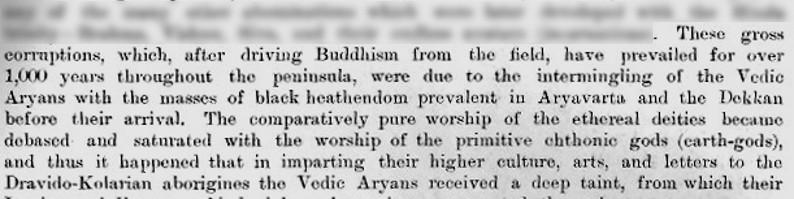
\includegraphics[scale=0.35]{"images/7-01.jpg"}
\caption{}\label{art7-fig01}
\end{figure}

In conclusion, it can be said that there is no such thing as an Aryan race. Consequently there are no “Dravidians” either as a separate “race” of people. These ideas were a fabrication that was necessary to construct a supremacist history in nineteenth century Europe.

Unfortunately this was the “knowledge” imparted to Indian schoolchildren as Indians started getting recruited by the British to work for British India. Aryans and Dravidians, who did not previously exist in the history or narrative of India, gradually became part of the Indian narrative and is now “accepted fact” among a large number of Indians as well as accepted scholarly wisdom in the west. It will be a very long time before this unfortunate lie can be wiped clean from the minds of misinformed Indians.


\section*{PART 2}

We will next look at the theory that Sanskrit, or a precursor language to Sanskrit was brought to India from somewhere outside India. As we have seen earlier, the “Aryan race” was an imaginary entity that was cooked up in order to claim that the language (Sanskrit, or a precursor of Sanskrit) was brought to India by an imagined people called Aryans. What is the evidence offered by linguists, historians and archaeologists to support this idea of “movement of language to India from somewhere outside.”

It will be seen that all the efforts to create a story in which language comes to India from outside revolve around linking individual words or passages from the Vedas to events or archaeological finds outside India. Mysteriously, very few scholars have attempted to link words from texts to findings within India. The need to link Sanskrit to an outside source is has dominated the discourse.

In order to explain this curious anomaly one must know why Sanskrit became such an important language for Europeans; so important in fact that they wanted to claim some kind of connection with Sanskrit and went through all the trouble to make up theories of how the language appeared in India.

When European scholars studied Sanskrit texts, they were surprised to discover the similarity of Sanskrit to European languages like Latin, French, German and English. Even more significant was the discovery by Europeans of Sanskrit grammar. Until then, European linguists knew that their own languages in Europe were somewhat similar, but it was the revelation of Sanskrit grammar that made them aware of how and why European languages were related.

Max Müller wrote: (index Muller, Max)

\begin{myquote}
‘The world had known Latin and Greek for centuries, and it was felt, no doubt, that there was some kind of similarity between the two. But how was that similarity to be explained? [...] But how such a likeness between these languages came to be, and how, what is far more difficult to explain, such striking differences too between these languages came to be, remained a mystery..[...] As soon, however, as Sanskrit stepped into the midst of these languages, there came light and warmth and mutual recognition.’ (Müller 1883:15)
\end{myquote}

Initially European “philologists” thought that Sanskrit may be the mother language of European languages (Huxley 1890). Translations of Sanskrit works into European languages threw up the word “Arya” or “Noble people” European scholars did not find it necessary to include the idea that “Arya” referred to noble people who strictly followed the traditions of Hindu Dharma. To European philologists “Arya” simply indicated a superior race members of which were dubbed “Aryans”. And that superior race could not be coffee or chocolate coloured Indians. From this was born the idea that “Aryans” came from the west, bringing a superior language and grammar to India where it had to be protected from the degradations that it was exposed to by the black Dravidians. 

\newpage

An imaginary history was written for Indians that the caste system was created by the migrant fair-skinned Aryans from Europe to protect their knowledge from dark skinned natives. Despite that, over centuries the superior Aryans in India interbred with the black people producing the “degraded” modern races of India (Huxley 1890: 5; Johnston 1902: 263). So the story grew that great white races from Europe came to India, defeated Dravidians and sent them south and settled in India but gradually degenerated into current day Indians who were not equal to white skinned Aryans. These theories, over time, came to be accepted as true and filled up scholarly textbooks making superior “Aryans”, the speakers of “Indo-Aryan languages” and dark skinned “Dravidians”, speakers of “Dravidian languages” an accepted “scientific” fact.

The finding of Sanskrit proper names and Vedic deities in Syria in the form of the Mitanni treaty tablets dating from 1700 BC was grabbed eagerly by German Assyriologists as proof that the Sanskrit language, on its way from Europe to India with victorious Aryan armies had stopped over briefly in Syria. The Semitic people of Assyria could not possibly have ruled their empire without the involvement of the superior Aryans from Europe (Frahm 2006: 85), who later made their way to India.

Despite all these constructions of “proof” for the story in which a mother language travels from Europe to India it turns out that there is no linguistic proof available from the points of origin either in Europe or Eurasia. The theory is all about language and people who spoke a language, but none of the starting points of migration have offered any proof of the language spoken when people started their journey towards India. Their language is simply assumed to be a precursor of Sanskrit. Sanskrit existed in India as a language handed down orally, with no written texts and there were no European written texts of adequate antiquity for comparison. In every instance individual mistranslated words and verses from the Vedas (Vidyarthi 1893:17-28) have been used to make a connection with archaeological finds (Anthony 2007:409) in places where there is no proof of the ancient language that was spoken in that remote past era. That language has simply been imagined to have been spoken by the people in the area in that pre-historic era, and later “reconstructed” by linguists.

\newpage

Because all efforts to try and find a “route of spread” of languages have centered around archaeological finds in the imagined “point of origin” of language in Europe or Eurasia and linking those finds to words from Sanskrit texts as the end point in India, the dates for the Rig Veda are frozen around the 1500 to 1000 BC period. This is simply because the relevant archaeological finds in Europe or Eurasia happen to be from around 2000 to 3000 BC and a 1000 year time gap is “allowed” for people to migrate to India where Sanskrit, the most developed Indo-European language, was “finally found.”

These dates can be falsified by an emergent new evidence – some of which point to dates as remote as 8000 BC, but the 1500 BC dates fixed by early philologists like Müller and contemporary anthropologist-historians like David Anthony (Anthony 2007: 82) have entered the mainstream body of knowledge along with the myth of an invasion or migration of “Aryans”. No one seems to want to “rock the boat” by looking at other, possibly older dates for the Vedas which are increasingly becoming likely from the work of a large body of new Indology researchers in India (Oak 2011; Sastry 2017). Older dates for the Vedas will require a complete re-thinking of the theory of language spread and would result in a revolutionary upsetting of fossilized 200 year old dogmatic claims about the origins of Indo-European languages. Once again parochial considerations among historians, linguists and scholars has led to the dismissal of new Indology studies as being motivated by Hindu revivalism or revisionism. Such accusations are reminiscent of the manner in which the medieval Catholic Church in Europe looked at any new information that threatened the dominance of the church narrative.


\section*{Part 3: Genetics}

There is a fundamental flaw in the search for genetic evidence of migration because many genetics papers start off with a tacit acceptance of the 1500 to 1000 BC dates for the language of the Vedas, assuming that it was brought to India by migrating Aryans. Consequently many researchers go about looking for migrations around those dates as possible evidence of the Aryan Migration Theory. This is an unfortunate consequence of the “Aryan Migration” theory having achieved mainstream status despite its sordid origins.

Genetic findings conclusively prove that there have been numerous migrations into India. There is no denying that. But genetics also shows migrations out of India. There have been migrations into India over 60,000 years ago, also over 12,000 years ago, and even 4,000 years ago and later. But linguists and historians are obsessed with the ‘4,000 ybp’ date because it fits in with their theory of victorious horse riding Aryans coming to India. Even contemporary scholars who reject the racist term “Aryan”, such as David Anthony who are stuck with linguistic “horse evidence” from mistranslations of the Vedas (Vidyarthi 1893: 17-28, Kashyap 2012: 55) finally narrow down on these relatively recent dates.

Migrations that may have occurred 12,000 years ago are too early for the language migration theory; 3000 years ago is too late. This is the only reason for attempting to zero in on genetic evidence of migrations into India in the 1500 to 1000 BC period. However genes do not provide any evidence of the language people spoke. There are no “language genes” just like there are no “Aryan genes”. Genetics alone can never provide direct proof of language and will not make any difference to the existing hurdles in the dating of languages. The Vedas have no dates – so all links are speculative.

Two seminal genetics papers (Reich 2009: 489–494; Tamang 2012: 911–919) threw an academic bombshell on migration theories focusing on the 1500 BC era. This study showed that all Indians in the subcontinent, starting from Kashmiri Pandits to tribals of Orissa, Karnataka and Tamil Nadu have a remarkably constant mix of unique “Indian” genes which have been given the name “Ancestral North Indian” (ASI) and “Ancestral South Indian” (ASI). Included in this study were Sindhis from Pakistan and Pathans from the Afghanistan-Pakistan region – who also carry the ANI+ASI gene mix like all Indians. Both the ASI and ANI components are very ancient genetic signatures. A migration out of Africa along the coast 65,000 years ago brought in the Ancestral South Indian genes, and a later migration 45,000 years ago were a set of genes among people who migrated out of Africa towards the Middle East, from where a branch went off to Europe and another branch came to India as “Ancestral North Indian” genes. (Fig 2)

\begin{figure}[!htbp]
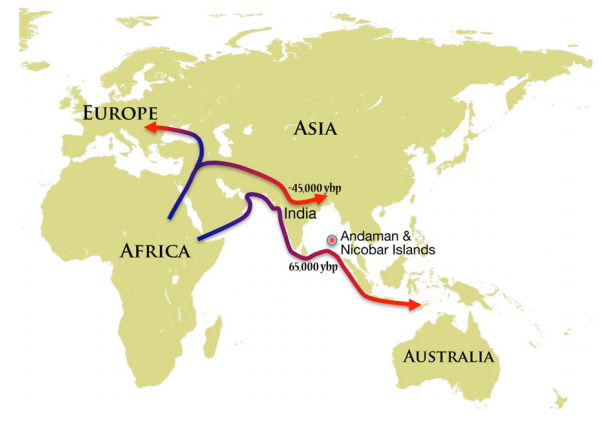
\includegraphics[scale=1.2]{"images/7-02.jpg"}
\caption{Image from (Tamang, Rakesh., Lalji Singh and Kumarasamy Thangaraj 2012: 911–919)}\label{art7-fig02}
\end{figure}

Every Indian carries a thorough mix of ASI and ANI genes and this gene mixture is unique to Indians. Indo-European language speakers (e.g.: Hindi, Bengali, Gujarati) carry about 45 to 60 \% ANI genes. South Indian language (“Dravidian language”) speakers carry 43 to 55\% ANI genes. The balance is ASI genes in each case. All in all, every Indian, whether forward caste, backward caste, Indo-European speaker or Dravidian language speaker carries approximately equal proportions of Ancestral North Indian and Ancestral South Indian genes. Even the only “outliers,” Pathans and Kashmiri Pandits carry 70\% ANI and 30\% ASI markers.

These findings throw great doubt on the theory that people carrying an Indo-European language migrated to India, driving Dravidians south and creating an upper caste that avoided mixing with lower castes to preserve the knowledge. Even Pathans and Kashmiri Pandits have 30\% Ancestral South Indian genes otherwise found among tribals of South India such as Chenchu and Onge. And those tribal groups show a greater than 40\% component “Ancestral North Indian” genes - genes which they should not have at all according to the Aryan migration/invasion theory. All other Indians show an approximate 60: 40 (or vice versa) mix of the two gene sets. Another paper (Metspalu 2011:731–744) showed that the ANI genes among Indians are older than would be expected if they represented a migration from Europe or Eurasia in the last 4000 years. In fact the paper concludes that the genes carrying the ANI component entered India more than 12,500 years ago.

It would be a valid question to ask how, if at all, is the above information in conflict with the Aryan invasion/migration theory (AIT/AMT)?

First, the papers negate the idea that Indo-European speakers created a system (caste system) that avoided interbreeding with “Dravidians” to help maintain the purity of an Aryan race. The thorough and complete admixture of ASI and ANI genes among all Indians of all castes and language groups makes this claim unsupportable.

Secondly, linguists and historians have tried to place the AIT/AMT story in the 1500 BC period because that era fits in with other theories that have been created to link Sanskrit with European languages via archaeology. But the genetic signatures of migrations into India are far older than the 1500 BC date postulated in current language migration theories.

It must be emphasized that while there is clear genetic evidence of many migrations into India, some as far back as the last ice age that ended 10,000 years ago and some as late as 4000 years ago, none of these migrations carry any proof of what language the migrants spoke either in their country of origin or upon arrival in India. There is no reason to reject an earlier migration date as less relevant than the later date in the absence of any proof of the language that migrants spoke at their point of origin. The genetic evidence so far points to migrations into India that pre-date the 1500 BC era by several thousand years. In fact the thorough mixing of ASI and ANI genes among Indians would favour a more remote date of migration rather than a more recent one. But a date of migration that is earlier than 4000 years ago would negate all current theories of spread of Indo-European languages – because that date has been carefully selected to fit in with archaeological findings of horses and wheels in Eurasia and linking them to words for horse, chariot and wheel in the Vedas. If the language in India was shown to be older the language migration theory would collapse.

It would be absurd to imagine that the people who painted the images of the Bhimbetka cave paintings in modern day Madhya Pradesh as long as 30,000 years ago had no language. Looking at Figure 2 which shows likely migrations 45,000 years ago which took people both towards Europe and towards India, it would not be hard to imagine that the first origins of Indo-European languages came from those people over 40,000 years ago rather than the imagined Aryans 3500 years ago. And the people with the new language mixed with an even older group of people speaking the precursor to Dravidian languages. The Vedas can be dated by various means that are all out of context for this paper other than to point out that all reasonable dates for the Vedas turn out to be prior to 5000 BC, or 7000 years before the present. The need to fix language at a relatively recent date appears to be a kind of mental hurdle in depicting the history of human languages by linking it to an imaginary migration of imaginary people.

European philologists who were intent on trying to link up Indo-\break European languages with Sanskrit simply discarded Dravidian\break languages as an outside group while they imagined dates for migration of people speaking those Indo-European languages. While they did not have the genetic information we have today, they also failed to notice that a large percentage of words in Telugu, Kannada, Tamizh and Malayalam are Sanskritic in origin. The mixing of languages is as complete as the mixing of genes. The only idea that does not fit the available facts is the Aryan Invasion/Migration theory which needs to be discarded and wiped out from academic circles.


\section*{Conclusions}

\begin{enumerate}[{\rm 1)}]
\itemsep=0pt
\item There were no Aryans who migrated to India.

 \item Consequently there were no Dravidians for Aryans to defeat or chase away.

 \item “Aryan” and “Dravidian” were terms coined by racist 19th century philologists to suit their vision of European supremacist history.

 \item All current theories of migration of Indo-Euorpean languages are stuck on a date of about 1500 B.C.E. for the Vedas because of reasons extraneous to ancient Indian history.

 \item Genes do not indicate language spoken. No matter what migrations are shown by genetics, the language cannot be linked to genes.

 \item Genetics has shown that the genetic signature among Indo-European language speakers in India is far older than the 1500 BC date suggested by the Aryan migration theory.

 \item Theories about the spread of Indo-European languages will require radical revision based on findings in India rather than current theories based on archaeology outside India.

\end{enumerate}


\section*{Bibliography}

\begin{thebibliography}{99}
\bibitem{chap7-key01} Anthony, David W. (2007) \textit{The Horse, the Wheel and Language- How Bronze-age riders From the Eurasian Steppes Shaped the Modern world}. Princeton and Oxford: Princeton University Press.

 \bibitem{chap7-key02} Frahm, Eckhart (2006) In Holloway, Steven W. (Ed.) \textit{Orientalism, Assyriology and the Bible}. Sheffield: Phoenix Press. pp 74-94.

 \bibitem{chap7-key03} Gobineau, Arthur, comte de (1915). \textit{The Inequality of Human Races. }William Heinemann, London. \url{https://archive.org/details/inequalityofhuma00gobi}

 \bibitem{chap7-key04} Godwin, Joscelyn (1996). \textit{Arktos: The Polar Myth in Science, Symbolism, and Nazi Survival}. Kemton, Illinois: Adventures Unlimited Press. \url{https://books.google.co.in/books?id=26v0qQcI0vwC&pg=PA43&lpg=PA43&dq=a+most+prolific+race,+of+great+stature,+muscular+strength,+energy,&source=bl&ots=FA9-9Nee_V&sig=IpHxbLsKnLV-Yz7atPLrwpTU8y4&hl=en&sa=X&ved=0ahUKEwiu46yv7fbVAhWIOY8KHf83B98Q6AEIJzAA#v=onepage&q=a%20most%20prolific%20race%2C%20of%20great%20stature%2C%20muscular%20strength%2C%20energy%2C&f=false}

 \bibitem{chap7-key05} Huxley, L. (1890) “The Aryan Question and Pre-Historic Man”. Collected Essays VII \url{https://mathcs.clarku.edu/huxley/CE7/Aryan.html}

 \bibitem{chap7-key06} Johnston, Harry H., Lydekker, R., Keane, Dr A.H., Hutchinson, H.N., Savage Landor, A.H., Shufeldt, Longford, Dr R.W. (1902) \textit{The Living Races of Mankind. }London\textit{:} Hutchinson and Co. \url{ https://archive.org/details/livingracesofman01john}

 \bibitem{chap7-key07} Kashyap R.L (2012) \textit{Rig Veda Samhita – Mandala 10. }Bangalore: Sri Aurobindo Kapali Sastry Institute of Vedic Culture.

 \bibitem{chap7-key08} Metspalu, M, Romero, I.G., Bazayit, Y., Chaubey, G., Mallick, C.B., Hudjashov, G., Nelis, M., Magi, R., Metspalu, E., Remm, M., Ramasamy, P., Singh L, Thangaraj, K., Villems, R., Kivisilid, T. (2011). “Shared and Unique Components of Human Population Structure and Genome-Wide Signals of Positive Selection in South Asia.” \textit{The American Journal of Human Genetics} 89, 731–744, December 9, 2011. \url{https://www.ncbi.nlm.nih.gov/pmc/articles/PMC3234374/}

 \bibitem{chap7-key09} Müller, Friedrich Max (2007) \textit{India: What It Can Teach Us. }New York\textit{: }Funk \& Wagnalls. \url{https://suratiundhiyu.files.wordpress.com/2011/02/india-what-can-it-teach-us.pdf}

 \bibitem{chap7-key10} Oak, Nilesh Nilkanth (2011) \textit{When did the Mahabharata War Happen: The Mystery of Arundhati.} Danphe Incorporated.

 \bibitem{chap7-key11} Reich, D., Thangaraj, K., Patterson, N. Alkes L. Price, and Singh L. (2009) “Reconstructing Indian Population History.” \textit{Nature}. 2009 Sep 24; 461(7263): 489–494. \url{https://www.ncbi.nlm.nih.gov/pmc/articles/PMC2842210/}

 \bibitem{chap7-key12} Sastry, Shivshankar (2017) Unpublished work.

 \bibitem{chap7-key13} Sayce, A. H. (1889) “The Primitive Home of the Aryans.” \textit{Science}, Vol. 14, No. 337 (Jul. 19, 1889), pp. 38-42 Published by: American Association for the Advancement of Science. \url{http://www.jstor.org/stable/1762461}

 \bibitem{chap7-key14} Tamang, Rakesh, Singh L. and Thangaraj, K. (2012) “Complex genetic origin of Indian populations and its implications.” \textit{J. Biosci}. 37(5), November 2012, 911–919. \url{http://www.ias.ac.in/article/fulltext/jbsc/037/05/0911-0919}

 \bibitem{chap7-key15} Vidyarthi, Pandit Guru Datta, M.A. (1893) \textit{The Terminology of the Vedas and European Scholars.} Mufid-i-Am Press, Lahore. \url{https://archive.org/details/terminologyofved00vidy}

 \end{thebibliography}

